\chapter{Bilder und Listings}

In den folgenden drei Kapiteln wird der Autor eine einfache Webservice-Umgebung aufbauen, um zu zeigen, wie Webservices in der Praxis angeboten, konsumiert und orchestriert werden k�nnen. Hierzu verwendet er ausschlie�lich Open-Source-Software, im Speziellen \NeuerBegriff{Apache Tomcat}\footnote{Website: \url{http://tomcat.apache.org/}} als Servlet-Engine, \NeuerBegriff{Apache Axis2}\footnote{Website: \url{http://ws.apache.org/axis2/}} als SOAP-Engine und \NeuerBegriff{ActiveBPEL}\footnote{Website: \url{http://www.activebpel.org/}} als Workflow-System. Die Installation und Konfiguration der ben�tigten Anwendungen wird in Kapitel \ref{sec:Werkzeuge} beschrieben. Die komplette Umgebung inkl. der vom Autor erstellten Webservices befindet sich als virtuelle Maschine auf der dieser Arbeit beigelegten DVD. Im Folgenden wird der DNS-Name \Code{linux-ws} als Bezeichnung f�r den Webservice-Server verwendet.

\section{Anbieten eines Webservice}
\label{sec:AnbietenEinesWebservices}
Mit Hilfe von Apache Axis2 k�nnen Webservices sehr einfach auf Basis von normalen Java-Klassen angeboten werden. Es ist lediglich eine zus�tzliche XML-Datei namens \Datei{META-INF/services.xml} n�tig, in der die zu ver�ffentlichenden Klassen und Methoden beschrieben werden. \abbildung{HelloWorldStruktur} zeigt die Struktur eines einfachen \Webservice{HelloWorld}-Webservice.

\begin{figure}[htb]
\centering
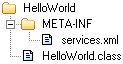
\includegraphics[width=0.3\textwidth]{HelloWorldStruktur.jpg}
\caption{\Webservice{HelloWorld}-Webservice: Dateistruktur}
\label{fig:HelloWorldStruktur}
\end{figure}

Die Klasse \Code{HelloWorld} besitzt nur die Methode \Code{SayHello}, die den \Datentyp{String} \Code{Hello World!} zur�ckgibt. Sie wird in Listing \ref{lst:HelloWorldJava} gezeigt. 

\newpage
\lstset{language=Java, basicstyle=\footnotesize, showstringspaces=false, tabsize=2}
\lstinputlisting[label=lst:HelloWorldJava,caption=\Webservice{HelloWorld}-Webservice: Java-Klasse \Code{HelloWorld}]{DVD/Listings/HelloWorld/HelloWorld.java}

\section{Netzwerkverkehr beim Aufruf von \Webservice{PersonFactory}}

\subsection{SOAP-Request}
Listing \ref{lst:SOAPRequest} zeigt die mitgeschnittene SOAP-Anfrage per HTTP an den Webservice \Webservice{PersonFactory}. Wie am Ende von Kapitel \ref{cha:Einleitung} beschrieben, wird die eigentliche SOAP-Nachricht mittels des HTTP-\Eingabe{POST}-Befehls (Zeile 1) an den Webservice unter der angegebenen URL (Zeile 1) auf dem Server (Zeile 5) geschickt. In Zeile 3 wird �ber den Befehl \Eingabe{SOAPAction} �bermittelt, welche Funktion des Webservice (in diesem Fall \Code{CreatePerson}) aufgerufen werden soll. Die XML-Nutzlast (Zeilen 8--18) besteht dann aus einer einfachen SOAP-Nachricht aus \XMLElement{Envelope}, \XMLElement{Header} und \XMLElement{Body}, die einen RPC durchf�hrt. Die aufzurufenden Funktion wird noch einmal im SOAP-\XMLElement{Body} in Zeile 15 definiert.


\lstset{language=XML, basicstyle=\footnotesize, showstringspaces=false, tabsize=2}
\lstinputlisting[label=lst:SOAPRequest,caption=SOAP-Request an \Webservice{PersonFactory} per HTTP]{DVD/Listings/PersonFactorySOAPRequest.txt}

\subsection{SOAP-Response}
Die Antwort des \Webservice{PersonFactory}-Webservice zeigt Listing \ref{lst:SOAPResponse}. Sie beginnt in Zeile 1 mit dem HTTP-Statuscode 200, der die Anfrage als erfolgreich kennzeichnet. Die eigentliche Nutzlast in Form von XML-Daten (Zeile 3) folgt dann ab Zeile 7. Sie besteht aus dem Element \XMLElement{Person} und seinen Unterelementen, umschlossen vom Element \XMLElement{CreatePersonRepsonse}, das die Antwort-Nachricht aus der WSDL repr�sentiert.

\lstset{language=XML, basicstyle=\footnotesize, showstringspaces=false, tabsize=2}
\lstinputlisting[label=lst:SOAPResponse,caption=SOAP-Response von \Webservice{PersonFactory} per HTTP]{DVD/Listings/PersonFactorySOAPResponse.txt}
